% Options for packages loaded elsewhere
\PassOptionsToPackage{unicode}{hyperref}
\PassOptionsToPackage{hyphens}{url}
%
\documentclass[
]{article}
\usepackage{amsmath,amssymb}
\usepackage{lmodern}
\usepackage{iftex}
\ifPDFTeX
  \usepackage[T1]{fontenc}
  \usepackage[utf8]{inputenc}
  \usepackage{textcomp} % provide euro and other symbols
\else % if luatex or xetex
  \usepackage{unicode-math}
  \defaultfontfeatures{Scale=MatchLowercase}
  \defaultfontfeatures[\rmfamily]{Ligatures=TeX,Scale=1}
\fi
% Use upquote if available, for straight quotes in verbatim environments
\IfFileExists{upquote.sty}{\usepackage{upquote}}{}
\IfFileExists{microtype.sty}{% use microtype if available
  \usepackage[]{microtype}
  \UseMicrotypeSet[protrusion]{basicmath} % disable protrusion for tt fonts
}{}
\makeatletter
\@ifundefined{KOMAClassName}{% if non-KOMA class
  \IfFileExists{parskip.sty}{%
    \usepackage{parskip}
  }{% else
    \setlength{\parindent}{0pt}
    \setlength{\parskip}{6pt plus 2pt minus 1pt}}
}{% if KOMA class
  \KOMAoptions{parskip=half}}
\makeatother
\usepackage{xcolor}
\usepackage[margin=1in]{geometry}
\usepackage{color}
\usepackage{fancyvrb}
\newcommand{\VerbBar}{|}
\newcommand{\VERB}{\Verb[commandchars=\\\{\}]}
\DefineVerbatimEnvironment{Highlighting}{Verbatim}{commandchars=\\\{\}}
% Add ',fontsize=\small' for more characters per line
\usepackage{framed}
\definecolor{shadecolor}{RGB}{248,248,248}
\newenvironment{Shaded}{\begin{snugshade}}{\end{snugshade}}
\newcommand{\AlertTok}[1]{\textcolor[rgb]{0.94,0.16,0.16}{#1}}
\newcommand{\AnnotationTok}[1]{\textcolor[rgb]{0.56,0.35,0.01}{\textbf{\textit{#1}}}}
\newcommand{\AttributeTok}[1]{\textcolor[rgb]{0.77,0.63,0.00}{#1}}
\newcommand{\BaseNTok}[1]{\textcolor[rgb]{0.00,0.00,0.81}{#1}}
\newcommand{\BuiltInTok}[1]{#1}
\newcommand{\CharTok}[1]{\textcolor[rgb]{0.31,0.60,0.02}{#1}}
\newcommand{\CommentTok}[1]{\textcolor[rgb]{0.56,0.35,0.01}{\textit{#1}}}
\newcommand{\CommentVarTok}[1]{\textcolor[rgb]{0.56,0.35,0.01}{\textbf{\textit{#1}}}}
\newcommand{\ConstantTok}[1]{\textcolor[rgb]{0.00,0.00,0.00}{#1}}
\newcommand{\ControlFlowTok}[1]{\textcolor[rgb]{0.13,0.29,0.53}{\textbf{#1}}}
\newcommand{\DataTypeTok}[1]{\textcolor[rgb]{0.13,0.29,0.53}{#1}}
\newcommand{\DecValTok}[1]{\textcolor[rgb]{0.00,0.00,0.81}{#1}}
\newcommand{\DocumentationTok}[1]{\textcolor[rgb]{0.56,0.35,0.01}{\textbf{\textit{#1}}}}
\newcommand{\ErrorTok}[1]{\textcolor[rgb]{0.64,0.00,0.00}{\textbf{#1}}}
\newcommand{\ExtensionTok}[1]{#1}
\newcommand{\FloatTok}[1]{\textcolor[rgb]{0.00,0.00,0.81}{#1}}
\newcommand{\FunctionTok}[1]{\textcolor[rgb]{0.00,0.00,0.00}{#1}}
\newcommand{\ImportTok}[1]{#1}
\newcommand{\InformationTok}[1]{\textcolor[rgb]{0.56,0.35,0.01}{\textbf{\textit{#1}}}}
\newcommand{\KeywordTok}[1]{\textcolor[rgb]{0.13,0.29,0.53}{\textbf{#1}}}
\newcommand{\NormalTok}[1]{#1}
\newcommand{\OperatorTok}[1]{\textcolor[rgb]{0.81,0.36,0.00}{\textbf{#1}}}
\newcommand{\OtherTok}[1]{\textcolor[rgb]{0.56,0.35,0.01}{#1}}
\newcommand{\PreprocessorTok}[1]{\textcolor[rgb]{0.56,0.35,0.01}{\textit{#1}}}
\newcommand{\RegionMarkerTok}[1]{#1}
\newcommand{\SpecialCharTok}[1]{\textcolor[rgb]{0.00,0.00,0.00}{#1}}
\newcommand{\SpecialStringTok}[1]{\textcolor[rgb]{0.31,0.60,0.02}{#1}}
\newcommand{\StringTok}[1]{\textcolor[rgb]{0.31,0.60,0.02}{#1}}
\newcommand{\VariableTok}[1]{\textcolor[rgb]{0.00,0.00,0.00}{#1}}
\newcommand{\VerbatimStringTok}[1]{\textcolor[rgb]{0.31,0.60,0.02}{#1}}
\newcommand{\WarningTok}[1]{\textcolor[rgb]{0.56,0.35,0.01}{\textbf{\textit{#1}}}}
\usepackage{longtable,booktabs,array}
\usepackage{calc} % for calculating minipage widths
% Correct order of tables after \paragraph or \subparagraph
\usepackage{etoolbox}
\makeatletter
\patchcmd\longtable{\par}{\if@noskipsec\mbox{}\fi\par}{}{}
\makeatother
% Allow footnotes in longtable head/foot
\IfFileExists{footnotehyper.sty}{\usepackage{footnotehyper}}{\usepackage{footnote}}
\makesavenoteenv{longtable}
\usepackage{graphicx}
\makeatletter
\def\maxwidth{\ifdim\Gin@nat@width>\linewidth\linewidth\else\Gin@nat@width\fi}
\def\maxheight{\ifdim\Gin@nat@height>\textheight\textheight\else\Gin@nat@height\fi}
\makeatother
% Scale images if necessary, so that they will not overflow the page
% margins by default, and it is still possible to overwrite the defaults
% using explicit options in \includegraphics[width, height, ...]{}
\setkeys{Gin}{width=\maxwidth,height=\maxheight,keepaspectratio}
% Set default figure placement to htbp
\makeatletter
\def\fps@figure{htbp}
\makeatother
\setlength{\emergencystretch}{3em} % prevent overfull lines
\providecommand{\tightlist}{%
  \setlength{\itemsep}{0pt}\setlength{\parskip}{0pt}}
\setcounter{secnumdepth}{-\maxdimen} % remove section numbering
\usepackage{booktabs}
\usepackage{longtable}
\usepackage{array}
\usepackage{multirow}
\usepackage{wrapfig}
\usepackage{float}
\usepackage{colortbl}
\usepackage{pdflscape}
\usepackage{tabu}
\usepackage{threeparttable}
\usepackage{threeparttablex}
\usepackage[normalem]{ulem}
\usepackage{makecell}
\usepackage{xcolor}
\ifLuaTeX
  \usepackage{selnolig}  % disable illegal ligatures
\fi
\IfFileExists{bookmark.sty}{\usepackage{bookmark}}{\usepackage{hyperref}}
\IfFileExists{xurl.sty}{\usepackage{xurl}}{} % add URL line breaks if available
\urlstyle{same} % disable monospaced font for URLs
\hypersetup{
  pdftitle={Simulation Experiment Results},
  pdfauthor={Victor Tsang (z5209633)},
  hidelinks,
  pdfcreator={LaTeX via pandoc}}

\title{Simulation Experiment Results}
\author{Victor Tsang (z5209633)}
\date{2022-11-08}

\begin{document}
\maketitle

\hypertarget{load-in-the-results}{%
\subsubsection{Load in the results}\label{load-in-the-results}}

\begin{Shaded}
\begin{Highlighting}[]
\FunctionTok{library}\NormalTok{(knitr)}
\FunctionTok{library}\NormalTok{(tidyverse)}
\FunctionTok{library}\NormalTok{(latex2exp)}

\FunctionTok{load}\NormalTok{(}\StringTok{"../data/synthetic{-}data.RData"}\NormalTok{)}
\FunctionTok{attach}\NormalTok{(synthetic.data.config)}

\NormalTok{estimates }\OtherTok{=} \FunctionTok{readRDS}\NormalTok{(}\StringTok{"../data/sim\_exp{-}estimate\_extinction\_results.RDS"}\NormalTok{)}
\NormalTok{estimates }\OtherTok{=}\NormalTok{ estimates }\SpecialCharTok{\%\textgreater{}\%} \FunctionTok{filter}\NormalTok{(}\SpecialCharTok{!}\NormalTok{(method }\SpecialCharTok{\%in\%} \FunctionTok{c}\NormalTok{(}\StringTok{"SI{-}RM"}\NormalTok{, }\StringTok{"GB{-}RM"}\NormalTok{)))}
\NormalTok{estimates }\OtherTok{=}\NormalTok{ estimates }\SpecialCharTok{\%\textgreater{}\%} \FunctionTok{mutate}\NormalTok{(}\FunctionTok{across}\NormalTok{(method, str\_replace, }\StringTok{\textquotesingle{}SI{-}RM{-}corrected\textquotesingle{}}\NormalTok{, }\StringTok{\textquotesingle{}SI{-}RM\textquotesingle{}}\NormalTok{))}
\NormalTok{estimates }\OtherTok{=}\NormalTok{ estimates }\SpecialCharTok{\%\textgreater{}\%} \FunctionTok{mutate}\NormalTok{(}\AttributeTok{method\_cat =} \FunctionTok{ifelse}\NormalTok{(method }\SpecialCharTok{\%in\%} \FunctionTok{c}\NormalTok{(}\StringTok{"SI{-}RM"}\NormalTok{, }\StringTok{"MINMI"}\NormalTok{), }\StringTok{"Proposed"}\NormalTok{, }\StringTok{"Existing"}\NormalTok{))}
\FunctionTok{head}\NormalTok{(estimates)}
\end{Highlighting}
\end{Shaded}

\begin{verbatim}
##   id error_factor method     lower     point    upper point_runtime
## 1  1          0.0    MLE        NA 12660.896       NA  1.907349e-05
## 2  1          0.0 BA-MLE        NA 12293.940       NA  1.682997e-03
## 3  1          0.0 SI-UGM 11262.804 12422.265 12681.61  3.777524e+00
## 4  2          0.5    MLE        NA  9871.056       NA  1.279831e-03
## 5  2          0.5 BA-MLE        NA  9364.609       NA  4.145861e-03
## 6  2          0.5 SI-UGM  7789.998  9518.421 10035.51  2.695084e+00
##   conf_int_runtime method_cat
## 1               NA   Existing
## 2               NA   Existing
## 3         3.777524   Existing
## 4               NA   Existing
## 5               NA   Existing
## 6         2.695084   Existing
\end{verbatim}

\begin{Shaded}
\begin{Highlighting}[]
\CommentTok{\# Point estimates}
\NormalTok{performance.point\_estimates }\OtherTok{=}\NormalTok{ estimates }\SpecialCharTok{\%\textgreater{}\%}
  \FunctionTok{filter}\NormalTok{(}\SpecialCharTok{!}\FunctionTok{is.na}\NormalTok{(point)) }\SpecialCharTok{\%\textgreater{}\%}
  \FunctionTok{group\_by}\NormalTok{(error\_factor, method, method\_cat) }\SpecialCharTok{\%\textgreater{}\%}
  \FunctionTok{summarise}\NormalTok{(}\AttributeTok{MSE\_000 =} \FunctionTok{mean}\NormalTok{((point }\SpecialCharTok{{-}}\NormalTok{ theta.true)}\SpecialCharTok{\^{}}\DecValTok{2}\NormalTok{)}\SpecialCharTok{/}\DecValTok{1000}\NormalTok{,}
            \AttributeTok{bias =} \FunctionTok{mean}\NormalTok{(point)}\SpecialCharTok{{-}}\NormalTok{theta.true,}
            \AttributeTok{variance\_000 =} \FunctionTok{var}\NormalTok{(point)}\SpecialCharTok{/}\DecValTok{1000}\NormalTok{,}
            \AttributeTok{avg\_runtime =} \FunctionTok{mean}\NormalTok{(point\_runtime))}
\end{Highlighting}
\end{Shaded}

\begin{verbatim}
## `summarise()` has grouped output by 'error_factor', 'method'. You can override
## using the `.groups` argument.
\end{verbatim}

\begin{Shaded}
\begin{Highlighting}[]
\FunctionTok{kable}\NormalTok{(performance.point\_estimates)}
\end{Highlighting}
\end{Shaded}

\begin{longtable}[]{@{}
  >{\raggedleft\arraybackslash}p{(\columnwidth - 12\tabcolsep) * \real{0.1461}}
  >{\raggedright\arraybackslash}p{(\columnwidth - 12\tabcolsep) * \real{0.1798}}
  >{\raggedright\arraybackslash}p{(\columnwidth - 12\tabcolsep) * \real{0.1236}}
  >{\raggedleft\arraybackslash}p{(\columnwidth - 12\tabcolsep) * \real{0.1124}}
  >{\raggedleft\arraybackslash}p{(\columnwidth - 12\tabcolsep) * \real{0.1573}}
  >{\raggedleft\arraybackslash}p{(\columnwidth - 12\tabcolsep) * \real{0.1461}}
  >{\raggedleft\arraybackslash}p{(\columnwidth - 12\tabcolsep) * \real{0.1348}}@{}}
\toprule()
\begin{minipage}[b]{\linewidth}\raggedleft
error\_factor
\end{minipage} & \begin{minipage}[b]{\linewidth}\raggedright
method
\end{minipage} & \begin{minipage}[b]{\linewidth}\raggedright
method\_cat
\end{minipage} & \begin{minipage}[b]{\linewidth}\raggedleft
MSE\_000
\end{minipage} & \begin{minipage}[b]{\linewidth}\raggedleft
bias
\end{minipage} & \begin{minipage}[b]{\linewidth}\raggedleft
variance\_000
\end{minipage} & \begin{minipage}[b]{\linewidth}\raggedleft
avg\_runtime
\end{minipage} \\
\midrule()
\endhead
0.0 & BA-MLE & Existing & 234.5607 & -0.9379571 & 234.7946 &
0.0000219 \\
0.0 & GRIWM & Existing & 1183.5359 & -949.8850000 & 281.5360 &
2.3354816 \\
0.0 & GRIWM-corrected & Existing & 246.1900 & 133.7070000 & 228.5410 &
13.8988053 \\
0.0 & MINMI & Proposed & 247.4576 & 139.4092643 & 228.2509 &
0.0000110 \\
0.0 & MLE & Existing & 438.6601 & 475.2971837 & 212.9656 & 0.0000173 \\
0.0 & SI-RM & Proposed & 438.6601 & 475.2971837 & 212.9656 &
0.0310266 \\
0.0 & SI-UGM & Existing & 248.9648 & 150.6138962 & 226.5068 &
4.7065676 \\
0.0 & STRAUSS & Existing & 234.8453 & -0.7152842 & 235.0799 &
0.0000186 \\
0.5 & BA-MLE & Existing & 244.0353 & -22.0990141 & 243.7908 &
0.0000253 \\
0.5 & GRIWM & Existing & 1275.8894 & -992.6550000 & 290.8162 &
2.3588714 \\
0.5 & GRIWM-corrected & Existing & 244.7798 & 95.1730000 & 235.9578 &
13.8825358 \\
0.5 & MINMI & Proposed & 250.5532 & 115.4530742 & 237.4612 &
0.0004929 \\
0.5 & MLE & Existing & 428.0602 & 455.1437961 & 221.1254 & 0.0000192 \\
0.5 & SI-RM & Proposed & 428.0602 & 455.1437961 & 221.1254 &
0.0096979 \\
0.5 & SI-UGM & Existing & 250.7756 & 117.2579537 & 237.2634 &
2.3305912 \\
0.5 & STRAUSS & Existing & 245.5802 & -22.8493286 & 245.3034 &
0.0000224 \\
1.0 & BA-MLE & Existing & 365.6242 & -45.7554617 & 363.8946 &
0.0000216 \\
1.0 & GRIWM & Existing & 1547.7470 & -1060.0020000 & 424.5673 &
18.1072462 \\
1.0 & GRIWM-corrected & Existing & 345.2420 & 34.4120000 & 344.4022 &
13.9009544 \\
1.0 & MINMI & Proposed & 368.4990 & 100.8350222 & 358.6900 &
0.0005482 \\
1.0 & MLE & Existing & 516.8878 & 432.6138460 & 330.0631 & 0.0000176 \\
1.0 & SI-RM & Proposed & 516.8878 & 432.6138460 & 330.0631 &
0.0062744 \\
1.0 & SI-UGM & Existing & 371.3002 & 115.2129004 & 358.3845 &
1.9374115 \\
1.0 & STRAUSS & Existing & 366.4727 & -50.5383309 & 364.2829 &
0.0000187 \\
2.0 & BA-MLE & Existing & 542.9867 & -233.5215118 & 488.9434 &
0.0000210 \\
2.0 & GRIWM & Existing & 2506.9717 & -1407.5250000 & 526.3714 &
2.3640996 \\
2.0 & GRIWM-corrected & Existing & 504.9335 & -278.4774775 & 427.8120 &
13.9421990 \\
2.0 & MINMI & Proposed & 508.3236 & 20.6641924 & 508.4050 & 0.0005069 \\
2.0 & MLE & Existing & 507.4514 & 253.7890364 & 443.4860 & 0.0000176 \\
2.0 & SI-RM & Proposed & 507.4514 & 253.7890364 & 443.4860 &
0.0056648 \\
2.0 & SI-UGM & Existing & 501.5358 & 65.3780494 & 497.7593 &
1.6800792 \\
2.0 & STRAUSS & Existing & 553.8156 & -247.9251968 & 492.8416 &
0.0000189 \\
4.0 & BA-MLE & Existing & 1712.8705 & -817.7749246 & 1045.1599 &
0.0000204 \\
4.0 & GRIWM & Existing & 6714.4002 & -2401.1470000 & 949.8431 &
2.3609959 \\
4.0 & GRIWM-corrected & Existing & 2147.1454 & -1173.6520000 & 770.4568
& 14.0341402 \\
4.0 & MINMI & Proposed & 1171.7409 & -178.1210176 & 1141.1550 &
0.0005369 \\
4.0 & MLE & Existing & 1038.6355 & -302.6427854 & 947.9908 &
0.0000176 \\
4.0 & SI-RM & Proposed & 1038.6355 & -302.6427854 & 947.9908 &
0.0058391 \\
4.0 & SI-UGM & Existing & 1130.9207 & -28.3481103 & 1131.2483 &
1.3896884 \\
4.0 & STRAUSS & Existing & 1789.1141 & -862.4420005 & 1046.3543 &
0.0000193 \\
\bottomrule()
\end{longtable}

\begin{Shaded}
\begin{Highlighting}[]
\CommentTok{\# Confidence Intervals}
\NormalTok{performance.conf\_int\_estimates }\OtherTok{=}\NormalTok{ estimates }\SpecialCharTok{\%\textgreater{}\%}
  \FunctionTok{filter}\NormalTok{(}\SpecialCharTok{!}\FunctionTok{is.na}\NormalTok{(conf\_int\_runtime)) }\SpecialCharTok{\%\textgreater{}\%}
  \FunctionTok{mutate}\NormalTok{(}\AttributeTok{width =}\NormalTok{ upper }\SpecialCharTok{{-}}\NormalTok{ lower,}
         \AttributeTok{contains\_theta =} \FunctionTok{ifelse}\NormalTok{(theta.true }\SpecialCharTok{\textgreater{}}\NormalTok{ lower }\SpecialCharTok{\&}\NormalTok{ theta.true }\SpecialCharTok{\textless{}}\NormalTok{ upper, }\DecValTok{1}\NormalTok{, }\DecValTok{0}\NormalTok{)) }\SpecialCharTok{\%\textgreater{}\%}
  \FunctionTok{group\_by}\NormalTok{(error\_factor, method, method\_cat) }\SpecialCharTok{\%\textgreater{}\%}
  \FunctionTok{summarise}\NormalTok{(}\AttributeTok{Coverage =} \FunctionTok{mean}\NormalTok{(contains\_theta) }\SpecialCharTok{*} \DecValTok{100}\NormalTok{,}
            \StringTok{\textasciigrave{}}\AttributeTok{Average Width}\StringTok{\textasciigrave{}} \OtherTok{=} \FunctionTok{mean}\NormalTok{(width),}
            \StringTok{\textasciigrave{}}\AttributeTok{Average Runtime}\StringTok{\textasciigrave{}} \OtherTok{=} \FunctionTok{mean}\NormalTok{(conf\_int\_runtime)) }\SpecialCharTok{\%\textgreater{}\%}
  \FunctionTok{ungroup}\NormalTok{() }\SpecialCharTok{\%\textgreater{}\%}
  \FunctionTok{arrange}\NormalTok{(}\FunctionTok{desc}\NormalTok{(Coverage), }\StringTok{\textasciigrave{}}\AttributeTok{Average Width}\StringTok{\textasciigrave{}}\NormalTok{, }\StringTok{\textasciigrave{}}\AttributeTok{Average Runtime}\StringTok{\textasciigrave{}}\NormalTok{)}
\end{Highlighting}
\end{Shaded}

\begin{verbatim}
## `summarise()` has grouped output by 'error_factor', 'method'. You can override
## using the `.groups` argument.
\end{verbatim}

\begin{Shaded}
\begin{Highlighting}[]
\FunctionTok{kable}\NormalTok{(performance.conf\_int\_estimates)}
\end{Highlighting}
\end{Shaded}

\begin{longtable}[]{@{}
  >{\raggedleft\arraybackslash}p{(\columnwidth - 10\tabcolsep) * \real{0.1646}}
  >{\raggedright\arraybackslash}p{(\columnwidth - 10\tabcolsep) * \real{0.2025}}
  >{\raggedright\arraybackslash}p{(\columnwidth - 10\tabcolsep) * \real{0.1392}}
  >{\raggedleft\arraybackslash}p{(\columnwidth - 10\tabcolsep) * \real{0.1139}}
  >{\raggedleft\arraybackslash}p{(\columnwidth - 10\tabcolsep) * \real{0.1772}}
  >{\raggedleft\arraybackslash}p{(\columnwidth - 10\tabcolsep) * \real{0.2025}}@{}}
\toprule()
\begin{minipage}[b]{\linewidth}\raggedleft
error\_factor
\end{minipage} & \begin{minipage}[b]{\linewidth}\raggedright
method
\end{minipage} & \begin{minipage}[b]{\linewidth}\raggedright
method\_cat
\end{minipage} & \begin{minipage}[b]{\linewidth}\raggedleft
Coverage
\end{minipage} & \begin{minipage}[b]{\linewidth}\raggedleft
Average Width
\end{minipage} & \begin{minipage}[b]{\linewidth}\raggedleft
Average Runtime
\end{minipage} \\
\midrule()
\endhead
0.0 & SI-RM & Proposed & 97.60000 & 2054.552 & 0.0310266 \\
0.0 & SI-UGM & Existing & 97.30000 & 1961.144 & 4.7065676 \\
0.5 & SI-UGM & Existing & 96.20000 & 2091.093 & 2.3305912 \\
0.5 & MINMI & Proposed & 95.90000 & 2077.861 & 0.0012295 \\
2.0 & SI-UGM & Existing & 94.90000 & 2964.298 & 1.6800792 \\
4.0 & SI-UGM & Existing & 94.90000 & 4405.261 & 1.3896884 \\
2.0 & MINMI & Proposed & 94.70000 & 2932.730 & 0.0014222 \\
0.0 & MINMI & Proposed & 94.50000 & 1917.160 & 0.0000372 \\
4.0 & MINMI & Proposed & 94.10000 & 4342.911 & 0.0015463 \\
1.0 & SI-UGM & Existing & 93.70000 & 2351.533 & 1.9374115 \\
1.0 & MINMI & Proposed & 93.60000 & 2329.949 & 0.0013297 \\
4.0 & SI-RM & Proposed & 89.10000 & 3760.329 & 0.0058391 \\
2.0 & SI-RM & Proposed & 83.70000 & 2500.858 & 0.0056648 \\
2.0 & GRIWM-corrected & Existing & 80.58058 & 1949.667 & 13.9421990 \\
0.5 & SI-RM & Proposed & 80.30000 & 2375.394 & 0.0096979 \\
1.0 & SI-RM & Proposed & 79.40000 & 2459.189 & 0.0062744 \\
4.0 & GRIWM-corrected & Existing & 69.90000 & 3647.415 & 14.0341402 \\
1.0 & GRIWM-corrected & Existing & 69.50000 & 1047.995 & 13.9009544 \\
0.5 & GRIWM-corrected & Existing & 49.90000 & 548.084 & 13.8825358 \\
4.0 & GRIWM & Existing & 24.00000 & 4049.362 & 2.3609959 \\
2.0 & GRIWM & Existing & 22.60000 & 2163.503 & 2.3640996 \\
1.0 & GRIWM & Existing & 13.90000 & 1162.649 & 18.1072462 \\
0.5 & GRIWM & Existing & 7.00000 & 608.326 & 2.3588714 \\
0.0 & GRIWM & Existing & 0.00000 & 0.000 & 2.3354816 \\
0.0 & GRIWM-corrected & Existing & 0.00000 & 0.000 & 13.8988053 \\
\bottomrule()
\end{longtable}

\hypertarget{point-estimates}{%
\subsubsection{Point Estimates}\label{point-estimates}}

\begin{Shaded}
\begin{Highlighting}[]
\FunctionTok{library}\NormalTok{(kableExtra)}
\end{Highlighting}
\end{Shaded}

\begin{verbatim}
## Warning: package 'kableExtra' was built under R version 4.2.2
\end{verbatim}

\begin{verbatim}
## 
## Attaching package: 'kableExtra'
\end{verbatim}

\begin{verbatim}
## The following object is masked from 'package:dplyr':
## 
##     group_rows
\end{verbatim}

\begin{Shaded}
\begin{Highlighting}[]
\ControlFlowTok{for}\NormalTok{ (err }\ControlFlowTok{in}\NormalTok{ error\_factors) \{}
\NormalTok{  experiment.results.kbl }\OtherTok{=}\NormalTok{ performance.point\_estimates }\SpecialCharTok{\%\textgreater{}\%} 
    \FunctionTok{filter}\NormalTok{(error\_factor }\SpecialCharTok{==}\NormalTok{ err) }\SpecialCharTok{\%\textgreater{}\%} 
    \FunctionTok{ungroup}\NormalTok{() }\SpecialCharTok{\%\textgreater{}\%}
    \FunctionTok{mutate}\NormalTok{(}\FunctionTok{across}\NormalTok{(}\SpecialCharTok{!}\FunctionTok{c}\NormalTok{(method, avg\_runtime, method\_cat), round)) }\SpecialCharTok{\%\textgreater{}\%} 
    \FunctionTok{mutate}\NormalTok{(}\AttributeTok{avg\_runtime=}\FunctionTok{round}\NormalTok{(avg\_runtime, }\AttributeTok{digits=}\DecValTok{5}\NormalTok{)) }\SpecialCharTok{\%\textgreater{}\%}
    \FunctionTok{arrange}\NormalTok{(MSE\_000) }\SpecialCharTok{\%\textgreater{}\%}
    \FunctionTok{select}\NormalTok{(}\SpecialCharTok{{-}}\FunctionTok{c}\NormalTok{(error\_factor, method\_cat)) }\SpecialCharTok{\%\textgreater{}\%}
    \FunctionTok{kable}\NormalTok{(}\AttributeTok{booktabs=}\NormalTok{T, }\AttributeTok{col.names =} \FunctionTok{c}\NormalTok{(}\StringTok{""}\NormalTok{, }\StringTok{"(000\textquotesingle{}s years)"}\NormalTok{, }\StringTok{"(years)"}\NormalTok{, }\StringTok{"(000\textquotesingle{}s years)"}\NormalTok{, }\StringTok{"(seconds)"}\NormalTok{), }\AttributeTok{format=}\StringTok{"latex"}\NormalTok{) }\SpecialCharTok{\%\textgreater{}\%}
    \FunctionTok{add\_header\_above}\NormalTok{(}\FunctionTok{c}\NormalTok{(}\StringTok{"Method"} \OtherTok{=} \DecValTok{1}\NormalTok{, }\StringTok{"MSE"} \OtherTok{=} \DecValTok{1}\NormalTok{, }\StringTok{"Bias"}\OtherTok{=}\DecValTok{1}\NormalTok{, }\StringTok{"Variance"}\OtherTok{=}\DecValTok{1}\NormalTok{, }\StringTok{"Average Runtime"}\OtherTok{=}\DecValTok{1}\NormalTok{))}
  \FunctionTok{writeLines}\NormalTok{(experiment.results.kbl, }\FunctionTok{paste0}\NormalTok{(}\StringTok{"../figures/table{-}sim{-}exp{-}point{-}error"}\NormalTok{, err, }\StringTok{".tex"}\NormalTok{))}
  \FunctionTok{print}\NormalTok{(experiment.results.kbl)}
\NormalTok{\}}
\end{Highlighting}
\end{Shaded}

\begin{tabular}{lrrrr}
\toprule
\multicolumn{1}{c}{Method} & \multicolumn{1}{c}{MSE} & \multicolumn{1}{c}{Bias} & \multicolumn{1}{c}{Variance} & \multicolumn{1}{c}{Average Runtime} \\
\cmidrule(l{3pt}r{3pt}){1-1} \cmidrule(l{3pt}r{3pt}){2-2} \cmidrule(l{3pt}r{3pt}){3-3} \cmidrule(l{3pt}r{3pt}){4-4} \cmidrule(l{3pt}r{3pt}){5-5}
 & (000's years) & (years) & (000's years) & (seconds)\\
\midrule
BA-MLE & 235 & -1 & 235 & 0.00002\\
STRAUSS & 235 & -1 & 235 & 0.00002\\
GRIWM-corrected & 246 & 134 & 229 & 13.89881\\
MINMI & 247 & 139 & 228 & 0.00001\\
SI-UGM & 249 & 151 & 227 & 4.70657\\
\addlinespace
MLE & 439 & 475 & 213 & 0.00002\\
SI-RM & 439 & 475 & 213 & 0.03103\\
GRIWM & 1184 & -950 & 282 & 2.33548\\
\bottomrule
\end{tabular}

\begin{tabular}{lrrrr}
\toprule
\multicolumn{1}{c}{Method} & \multicolumn{1}{c}{MSE} & \multicolumn{1}{c}{Bias} & \multicolumn{1}{c}{Variance} & \multicolumn{1}{c}{Average Runtime} \\
\cmidrule(l{3pt}r{3pt}){1-1} \cmidrule(l{3pt}r{3pt}){2-2} \cmidrule(l{3pt}r{3pt}){3-3} \cmidrule(l{3pt}r{3pt}){4-4} \cmidrule(l{3pt}r{3pt}){5-5}
 & (000's years) & (years) & (000's years) & (seconds)\\
\midrule
BA-MLE & 244 & -22 & 244 & 0.00003\\
GRIWM-corrected & 245 & 95 & 236 & 13.88254\\
STRAUSS & 246 & -23 & 245 & 0.00002\\
MINMI & 251 & 115 & 237 & 0.00049\\
SI-UGM & 251 & 117 & 237 & 2.33059\\
\addlinespace
MLE & 428 & 455 & 221 & 0.00002\\
SI-RM & 428 & 455 & 221 & 0.00970\\
GRIWM & 1276 & -993 & 291 & 2.35887\\
\bottomrule
\end{tabular}

\begin{tabular}{lrrrr}
\toprule
\multicolumn{1}{c}{Method} & \multicolumn{1}{c}{MSE} & \multicolumn{1}{c}{Bias} & \multicolumn{1}{c}{Variance} & \multicolumn{1}{c}{Average Runtime} \\
\cmidrule(l{3pt}r{3pt}){1-1} \cmidrule(l{3pt}r{3pt}){2-2} \cmidrule(l{3pt}r{3pt}){3-3} \cmidrule(l{3pt}r{3pt}){4-4} \cmidrule(l{3pt}r{3pt}){5-5}
 & (000's years) & (years) & (000's years) & (seconds)\\
\midrule
GRIWM-corrected & 345 & 34 & 344 & 13.90095\\
BA-MLE & 366 & -46 & 364 & 0.00002\\
STRAUSS & 366 & -51 & 364 & 0.00002\\
MINMI & 368 & 101 & 359 & 0.00055\\
SI-UGM & 371 & 115 & 358 & 1.93741\\
\addlinespace
MLE & 517 & 433 & 330 & 0.00002\\
SI-RM & 517 & 433 & 330 & 0.00627\\
GRIWM & 1548 & -1060 & 425 & 18.10725\\
\bottomrule
\end{tabular}

\begin{tabular}{lrrrr}
\toprule
\multicolumn{1}{c}{Method} & \multicolumn{1}{c}{MSE} & \multicolumn{1}{c}{Bias} & \multicolumn{1}{c}{Variance} & \multicolumn{1}{c}{Average Runtime} \\
\cmidrule(l{3pt}r{3pt}){1-1} \cmidrule(l{3pt}r{3pt}){2-2} \cmidrule(l{3pt}r{3pt}){3-3} \cmidrule(l{3pt}r{3pt}){4-4} \cmidrule(l{3pt}r{3pt}){5-5}
 & (000's years) & (years) & (000's years) & (seconds)\\
\midrule
SI-UGM & 502 & 65 & 498 & 1.68008\\
GRIWM-corrected & 505 & -278 & 428 & 13.94220\\
MLE & 507 & 254 & 443 & 0.00002\\
SI-RM & 507 & 254 & 443 & 0.00566\\
MINMI & 508 & 21 & 508 & 0.00051\\
\addlinespace
BA-MLE & 543 & -234 & 489 & 0.00002\\
STRAUSS & 554 & -248 & 493 & 0.00002\\
GRIWM & 2507 & -1408 & 526 & 2.36410\\
\bottomrule
\end{tabular}

\begin{tabular}{lrrrr}
\toprule
\multicolumn{1}{c}{Method} & \multicolumn{1}{c}{MSE} & \multicolumn{1}{c}{Bias} & \multicolumn{1}{c}{Variance} & \multicolumn{1}{c}{Average Runtime} \\
\cmidrule(l{3pt}r{3pt}){1-1} \cmidrule(l{3pt}r{3pt}){2-2} \cmidrule(l{3pt}r{3pt}){3-3} \cmidrule(l{3pt}r{3pt}){4-4} \cmidrule(l{3pt}r{3pt}){5-5}
 & (000's years) & (years) & (000's years) & (seconds)\\
\midrule
MLE & 1039 & -303 & 948 & 0.00002\\
SI-RM & 1039 & -303 & 948 & 0.00584\\
SI-UGM & 1131 & -28 & 1131 & 1.38969\\
MINMI & 1172 & -178 & 1141 & 0.00054\\
BA-MLE & 1713 & -818 & 1045 & 0.00002\\
\addlinespace
STRAUSS & 1789 & -862 & 1046 & 0.00002\\
GRIWM-corrected & 2147 & -1174 & 770 & 14.03414\\
GRIWM & 6714 & -2401 & 950 & 2.36100\\
\bottomrule
\end{tabular}

\begin{Shaded}
\begin{Highlighting}[]
\FunctionTok{ggplot}\NormalTok{() }\SpecialCharTok{+}
  \FunctionTok{geom\_line}\NormalTok{(}\AttributeTok{data =} \FunctionTok{filter}\NormalTok{(performance.point\_estimates, method\_cat }\SpecialCharTok{==} \StringTok{"Existing"}\NormalTok{),}
            \FunctionTok{aes}\NormalTok{(}\AttributeTok{x=}\NormalTok{error\_factor, }\AttributeTok{group=}\NormalTok{method, }\AttributeTok{y=}\NormalTok{MSE\_000, }\AttributeTok{colour=}\NormalTok{method\_cat), }\AttributeTok{alpha=}\FloatTok{0.6}\NormalTok{) }\SpecialCharTok{+}
  \FunctionTok{geom\_line}\NormalTok{(}\AttributeTok{data =} \FunctionTok{filter}\NormalTok{(performance.point\_estimates, method\_cat }\SpecialCharTok{==} \StringTok{"Proposed"}\NormalTok{),}
            \FunctionTok{aes}\NormalTok{(}\AttributeTok{x=}\NormalTok{error\_factor, }\AttributeTok{y=}\NormalTok{MSE\_000, }\AttributeTok{colour=}\NormalTok{method)) }\SpecialCharTok{+}
  \FunctionTok{theme\_bw}\NormalTok{() }\SpecialCharTok{+}
  \FunctionTok{labs}\NormalTok{(}\AttributeTok{x=}\StringTok{"Error Factor"}\NormalTok{, }\AttributeTok{y=}\ConstantTok{NULL}\NormalTok{, }\AttributeTok{title=}\StringTok{"MSE (\textquotesingle{}000 years) of each Method"}\NormalTok{) }\SpecialCharTok{+}
  \FunctionTok{scale\_y\_continuous}\NormalTok{(}\AttributeTok{trans=}\StringTok{\textquotesingle{}log10\textquotesingle{}}\NormalTok{)}
\end{Highlighting}
\end{Shaded}

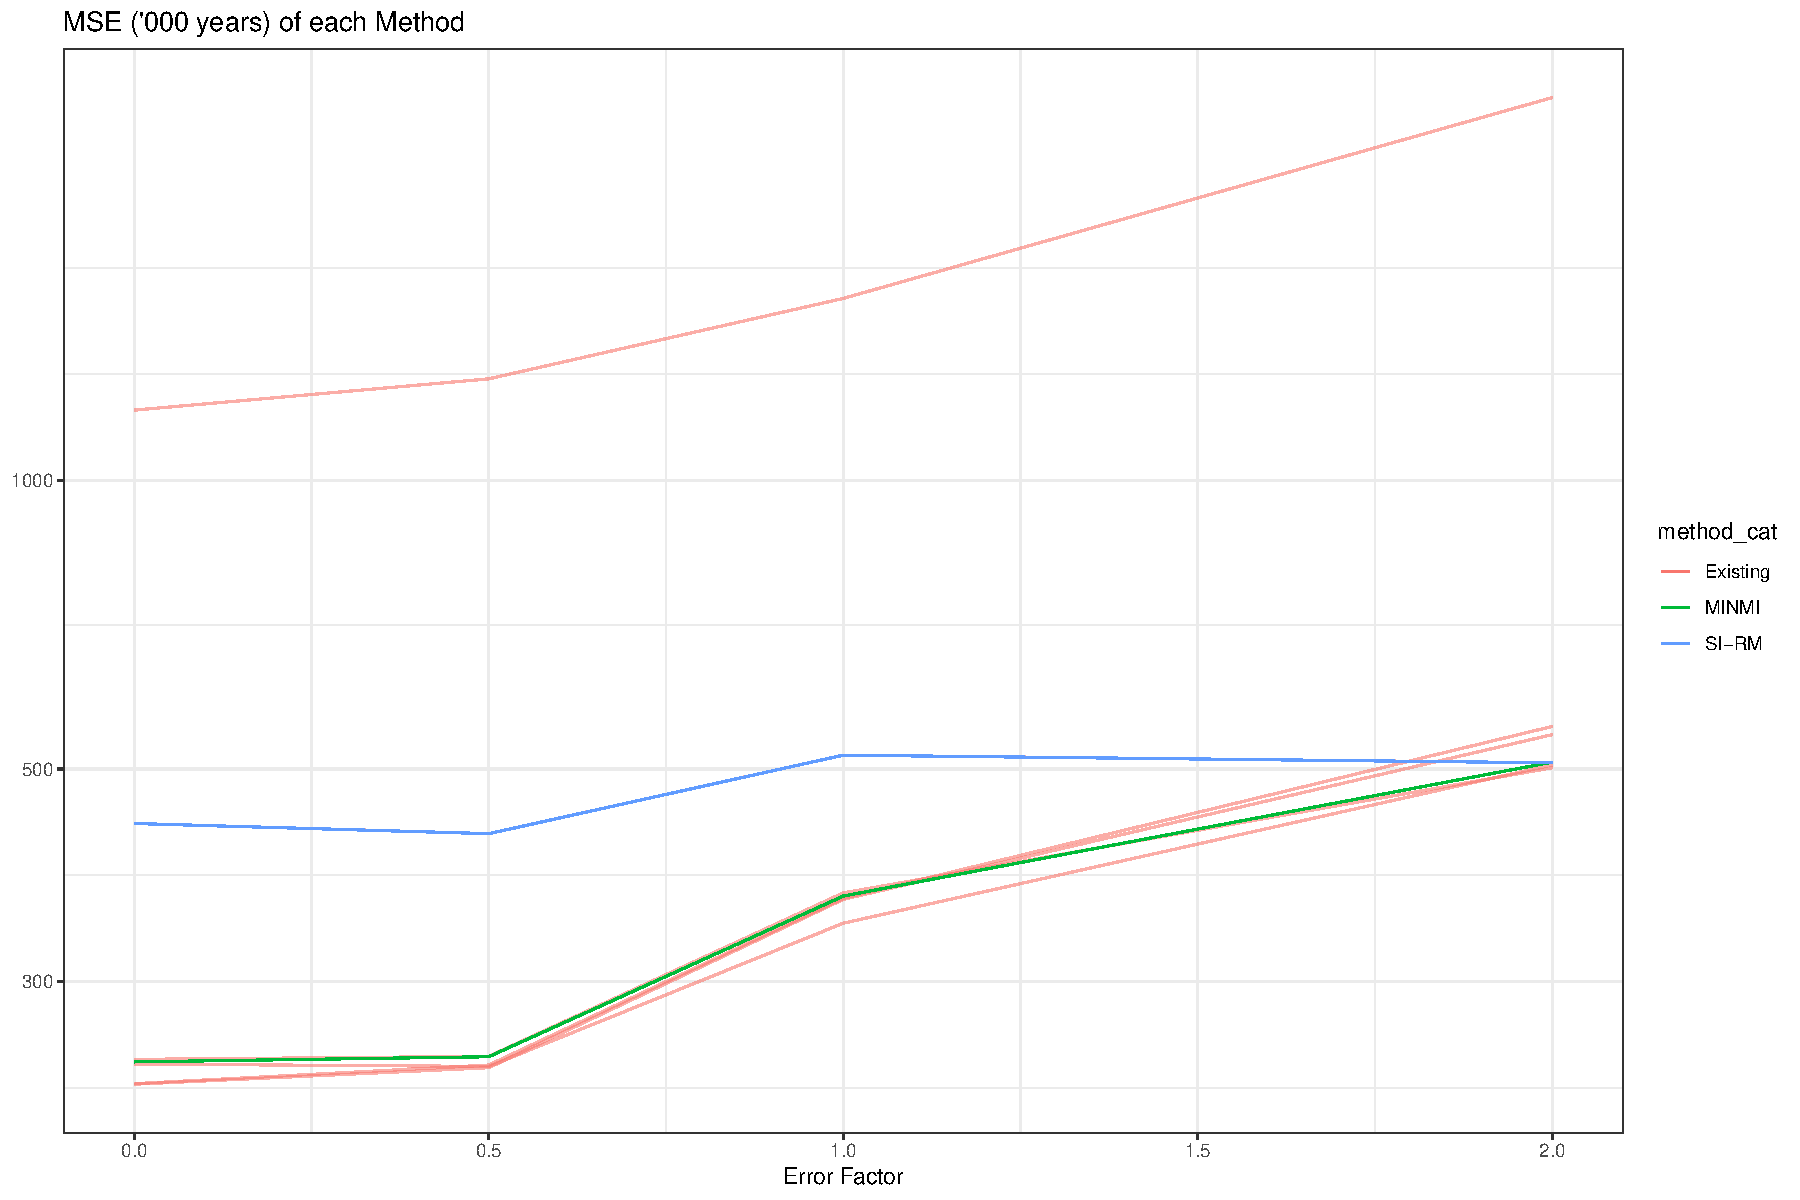
\includegraphics{sim_exp-results_files/figure-latex/unnamed-chunk-4-1.pdf}

\hypertarget{confidence-intervals}{%
\subsubsection{Confidence Intervals}\label{confidence-intervals}}

\begin{Shaded}
\begin{Highlighting}[]
\FunctionTok{options}\NormalTok{(}\AttributeTok{scipen=}\DecValTok{9}\NormalTok{)}
\ControlFlowTok{for}\NormalTok{ (metric }\ControlFlowTok{in} \FunctionTok{c}\NormalTok{(}\StringTok{"Coverage"}\NormalTok{, }\StringTok{"Average Width"}\NormalTok{, }\StringTok{"Average Runtime"}\NormalTok{)) \{}
\NormalTok{  experiment.results.kbl }\OtherTok{=}\NormalTok{ performance.conf\_int\_estimates }\SpecialCharTok{\%\textgreater{}\%}
    \FunctionTok{select}\NormalTok{(}\FunctionTok{c}\NormalTok{(method, error\_factor, }\FunctionTok{one\_of}\NormalTok{(metric))) }\SpecialCharTok{\%\textgreater{}\%}
    \FunctionTok{pivot\_wider}\NormalTok{(}\AttributeTok{id\_cols =}\NormalTok{ method,}
              \AttributeTok{names\_from=}\NormalTok{error\_factor,}
              \AttributeTok{values\_from=}\FunctionTok{one\_of}\NormalTok{(metric),}
              \AttributeTok{names\_prefix=}\FunctionTok{paste}\NormalTok{(metric, }\StringTok{"| error = sigma*"}\NormalTok{)) }\SpecialCharTok{\%\textgreater{}\%}
    \FunctionTok{arrange}\NormalTok{(}\SpecialCharTok{!!}\FunctionTok{syms}\NormalTok{(}\FunctionTok{paste}\NormalTok{(metric, }\StringTok{"| error = sigma*0"}\NormalTok{))) }\SpecialCharTok{\%\textgreater{}\%}
    \FunctionTok{kable}\NormalTok{(}\AttributeTok{booktabs=}\NormalTok{T, }\AttributeTok{col.names =} \FunctionTok{c}\NormalTok{(}\StringTok{"Method"}\NormalTok{, }\FunctionTok{paste0}\NormalTok{(}\FunctionTok{c}\NormalTok{(}\DecValTok{0}\NormalTok{,}\FloatTok{0.5}\NormalTok{,}\DecValTok{1}\NormalTok{,}\DecValTok{2}\NormalTok{,}\DecValTok{4}\NormalTok{), r}\StringTok{"\{*$\textbackslash{}sigma$\}"}\NormalTok{)), }\AttributeTok{format=}\StringTok{"latex"}\NormalTok{, }\AttributeTok{escape =} \ConstantTok{FALSE}\NormalTok{) }\SpecialCharTok{\%\textgreater{}\%}
    \CommentTok{\# kable\_styling(full\_width = F) \%\textgreater{}\%}
    \FunctionTok{add\_header\_above}\NormalTok{(}\FunctionTok{c}\NormalTok{(}\StringTok{" "} \OtherTok{=} \DecValTok{1}\NormalTok{, }\AttributeTok{metric =} \DecValTok{4}\NormalTok{))}
  
  \FunctionTok{print}\NormalTok{(experiment.results.kbl)}
  \FunctionTok{writeLines}\NormalTok{(experiment.results.kbl, }\FunctionTok{paste0}\NormalTok{(}\StringTok{"../figures/table{-}sim{-}exp{-}conf{-}int{-}"}\NormalTok{, }\FunctionTok{str\_replace}\NormalTok{(}\FunctionTok{tolower}\NormalTok{(metric), }\StringTok{" "}\NormalTok{, }\StringTok{"{-}"}\NormalTok{), }\StringTok{".tex"}\NormalTok{))}
\NormalTok{\}}
\end{Highlighting}
\end{Shaded}

\begin{tabular}{lrrrrr}
\toprule
\multicolumn{1}{c}{ } & \multicolumn{4}{c}{metric} \\
\cmidrule(l{3pt}r{3pt}){2-5}
Method & 0*$\sigma$ & 0.5*$\sigma$ & 1*$\sigma$ & 2*$\sigma$ & 4*$\sigma$\\
\midrule
SI-RM & 97.6 & 80.3 & 83.70000 & 89.1 & 79.4\\
SI-UGM & 97.3 & 96.2 & 94.90000 & 94.9 & 93.7\\
MINMI & 94.5 & 95.9 & 94.70000 & 94.1 & 93.6\\
GRIWM-corrected & 0.0 & 49.9 & 80.58058 & 69.9 & 69.5\\
GRIWM & 0.0 & 7.0 & 22.60000 & 24.0 & 13.9\\
\bottomrule
\end{tabular}

\begin{tabular}{lrrrrr}
\toprule
\multicolumn{1}{c}{ } & \multicolumn{4}{c}{metric} \\
\cmidrule(l{3pt}r{3pt}){2-5}
Method & 0*$\sigma$ & 0.5*$\sigma$ & 1*$\sigma$ & 2*$\sigma$ & 4*$\sigma$\\
\midrule
SI-RM & 2054.552 & 2375.394 & 2500.858 & 3760.329 & 2459.189\\
SI-UGM & 1961.144 & 2091.093 & 2964.298 & 4405.261 & 2351.533\\
MINMI & 1917.160 & 2077.861 & 2932.730 & 4342.911 & 2329.949\\
GRIWM-corrected & 0.000 & 548.084 & 1949.667 & 3647.415 & 1047.995\\
GRIWM & 0.000 & 608.326 & 2163.503 & 4049.362 & 1162.649\\
\bottomrule
\end{tabular}

\begin{tabular}{lrrrrr}
\toprule
\multicolumn{1}{c}{ } & \multicolumn{4}{c}{metric} \\
\cmidrule(l{3pt}r{3pt}){2-5}
Method & 0*$\sigma$ & 0.5*$\sigma$ & 1*$\sigma$ & 2*$\sigma$ & 4*$\sigma$\\
\midrule
SI-RM & 0.0310266 & 0.0096979 & 0.0056648 & 0.0058391 & 0.0062744\\
SI-UGM & 4.7065676 & 2.3305912 & 1.6800792 & 1.3896884 & 1.9374115\\
MINMI & 0.0000372 & 0.0012295 & 0.0014222 & 0.0015463 & 0.0013297\\
GRIWM-corrected & 13.8988053 & 13.8825358 & 13.9421990 & 14.0341402 & 13.9009544\\
GRIWM & 2.3354816 & 2.3588714 & 2.3640996 & 2.3609959 & 18.1072462\\
\bottomrule
\end{tabular}

\begin{Shaded}
\begin{Highlighting}[]
\NormalTok{estimates }\SpecialCharTok{\%\textgreater{}\%}
  \FunctionTok{filter}\NormalTok{(}\SpecialCharTok{!}\FunctionTok{is.na}\NormalTok{(lower)) }\SpecialCharTok{\%\textgreater{}\%}
  \FunctionTok{select}\NormalTok{(method, lower, upper) }\SpecialCharTok{\%\textgreater{}\%}
  \FunctionTok{pivot\_longer}\NormalTok{(}\AttributeTok{cols=}\FunctionTok{c}\NormalTok{(lower, upper)) }\SpecialCharTok{\%\textgreater{}\%}
  \FunctionTok{filter}\NormalTok{(}\SpecialCharTok{!}\FunctionTok{is.na}\NormalTok{(value)) }\SpecialCharTok{\%\textgreater{}\%}
  \FunctionTok{ggplot}\NormalTok{(}\FunctionTok{aes}\NormalTok{(}\AttributeTok{x=}\NormalTok{value, }\AttributeTok{fill=}\NormalTok{name)) }\SpecialCharTok{+}
  \FunctionTok{geom\_density}\NormalTok{(}\AttributeTok{alpha=}\FloatTok{0.25}\NormalTok{) }\SpecialCharTok{+}
  \FunctionTok{geom\_vline}\NormalTok{(}\FunctionTok{aes}\NormalTok{(}\AttributeTok{xintercept=}\NormalTok{theta.true)) }\SpecialCharTok{+}
  \FunctionTok{facet\_wrap}\NormalTok{(method }\SpecialCharTok{\textasciitilde{}}\NormalTok{ ., }\AttributeTok{nrow=}\DecValTok{1}\NormalTok{) }\SpecialCharTok{+}
  \FunctionTok{theme\_minimal}\NormalTok{() }\SpecialCharTok{+}
  \FunctionTok{labs}\NormalTok{(}\AttributeTok{x=}\ConstantTok{NULL}\NormalTok{, }\AttributeTok{y=}\ConstantTok{NULL}\NormalTok{)}
\end{Highlighting}
\end{Shaded}

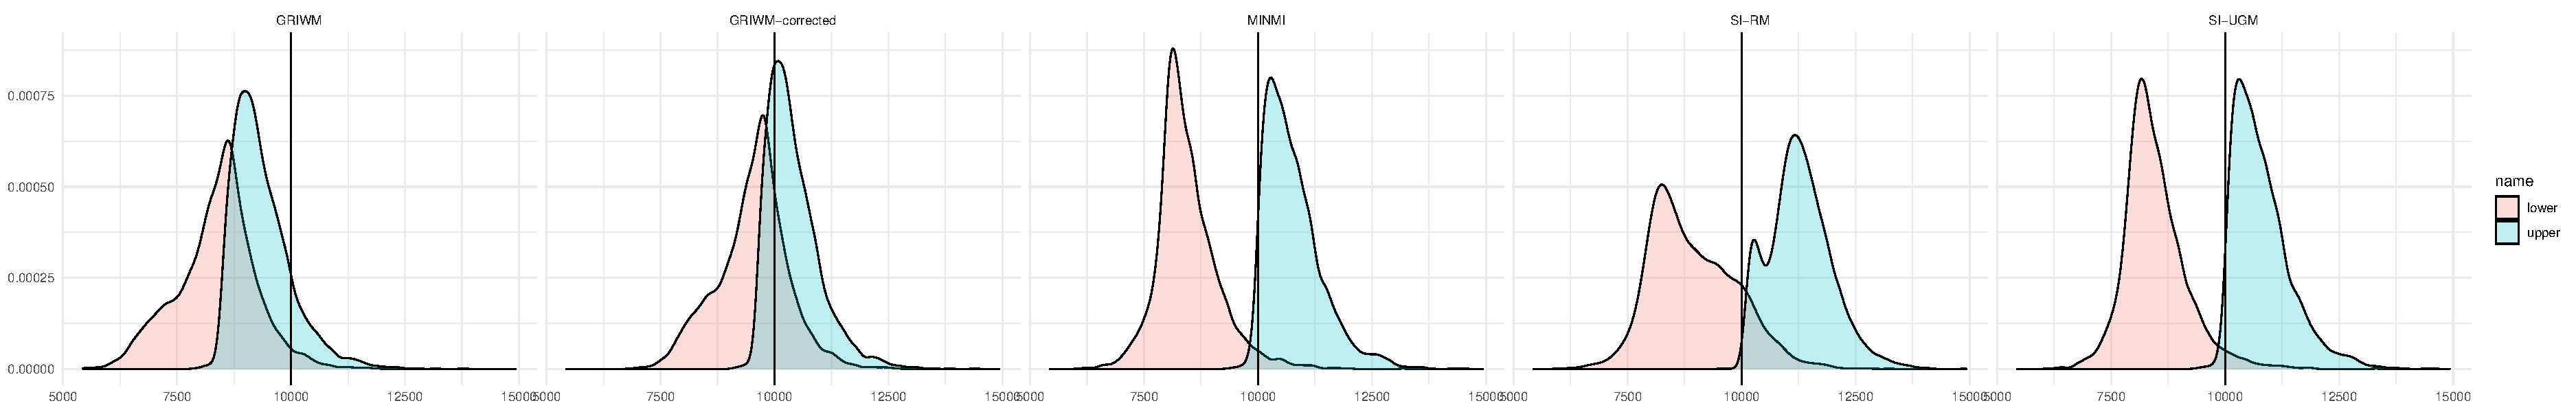
\includegraphics{sim_exp-results_files/figure-latex/unnamed-chunk-6-1.pdf}

\begin{Shaded}
\begin{Highlighting}[]
\NormalTok{estimates }\SpecialCharTok{\%\textgreater{}\%}
  \FunctionTok{filter}\NormalTok{(}\SpecialCharTok{!}\FunctionTok{is.na}\NormalTok{(lower) }\SpecialCharTok{\&}\NormalTok{ error\_factor }\SpecialCharTok{==} \DecValTok{1}\NormalTok{) }\SpecialCharTok{\%\textgreater{}\%}
  \FunctionTok{group\_by}\NormalTok{(method\_cat, method) }\SpecialCharTok{\%\textgreater{}\%}
  \FunctionTok{summarise}\NormalTok{(}\AttributeTok{lower =} \FunctionTok{mean}\NormalTok{(lower), }\AttributeTok{upper=}\FunctionTok{mean}\NormalTok{(upper)) }\SpecialCharTok{\%\textgreater{}\%}
  \FunctionTok{mutate}\NormalTok{(}\AttributeTok{width=}\NormalTok{upper}\SpecialCharTok{{-}}\NormalTok{lower) }\SpecialCharTok{\%\textgreater{}\%}
  \FunctionTok{mutate}\NormalTok{(}\AttributeTok{method\_cat\_int =} \FunctionTok{ifelse}\NormalTok{(method\_cat }\SpecialCharTok{==} \StringTok{"Existing"}\NormalTok{, }\DecValTok{0}\NormalTok{, }\DecValTok{1}\NormalTok{)) }\SpecialCharTok{\%\textgreater{}\%}
  \FunctionTok{ggplot}\NormalTok{(}\FunctionTok{aes}\NormalTok{(}\AttributeTok{y=}\FunctionTok{reorder}\NormalTok{(method, method\_cat\_int), }\AttributeTok{colour=}\NormalTok{method\_cat)) }\SpecialCharTok{+}
  \FunctionTok{geom\_errorbarh}\NormalTok{(}\FunctionTok{aes}\NormalTok{(}\AttributeTok{xmin=}\NormalTok{lower, }\AttributeTok{xmax=}\NormalTok{upper)) }\SpecialCharTok{+}
  \CommentTok{\# geom\_text(aes(y=method, x=(upper+lower)/2, label=round(width, 2)), vjust = {-}0.5) +}
  \FunctionTok{guides}\NormalTok{(}\AttributeTok{color =} \FunctionTok{guide\_legend}\NormalTok{(}\AttributeTok{reverse=}\ConstantTok{TRUE}\NormalTok{)) }\SpecialCharTok{+}
  \FunctionTok{labs}\NormalTok{(}\AttributeTok{x=}\ConstantTok{NULL}\NormalTok{, }\AttributeTok{y=}\StringTok{"Years (BP)"}\NormalTok{, }\AttributeTok{title=}\StringTok{"Simulation Experiment Confidence Intervals"}\NormalTok{, }\AttributeTok{colour=}\ConstantTok{NULL}\NormalTok{) }\SpecialCharTok{+}
  \FunctionTok{theme\_bw}\NormalTok{()}
\end{Highlighting}
\end{Shaded}

\begin{verbatim}
## `summarise()` has grouped output by 'method_cat'. You can override using the
## `.groups` argument.
\end{verbatim}

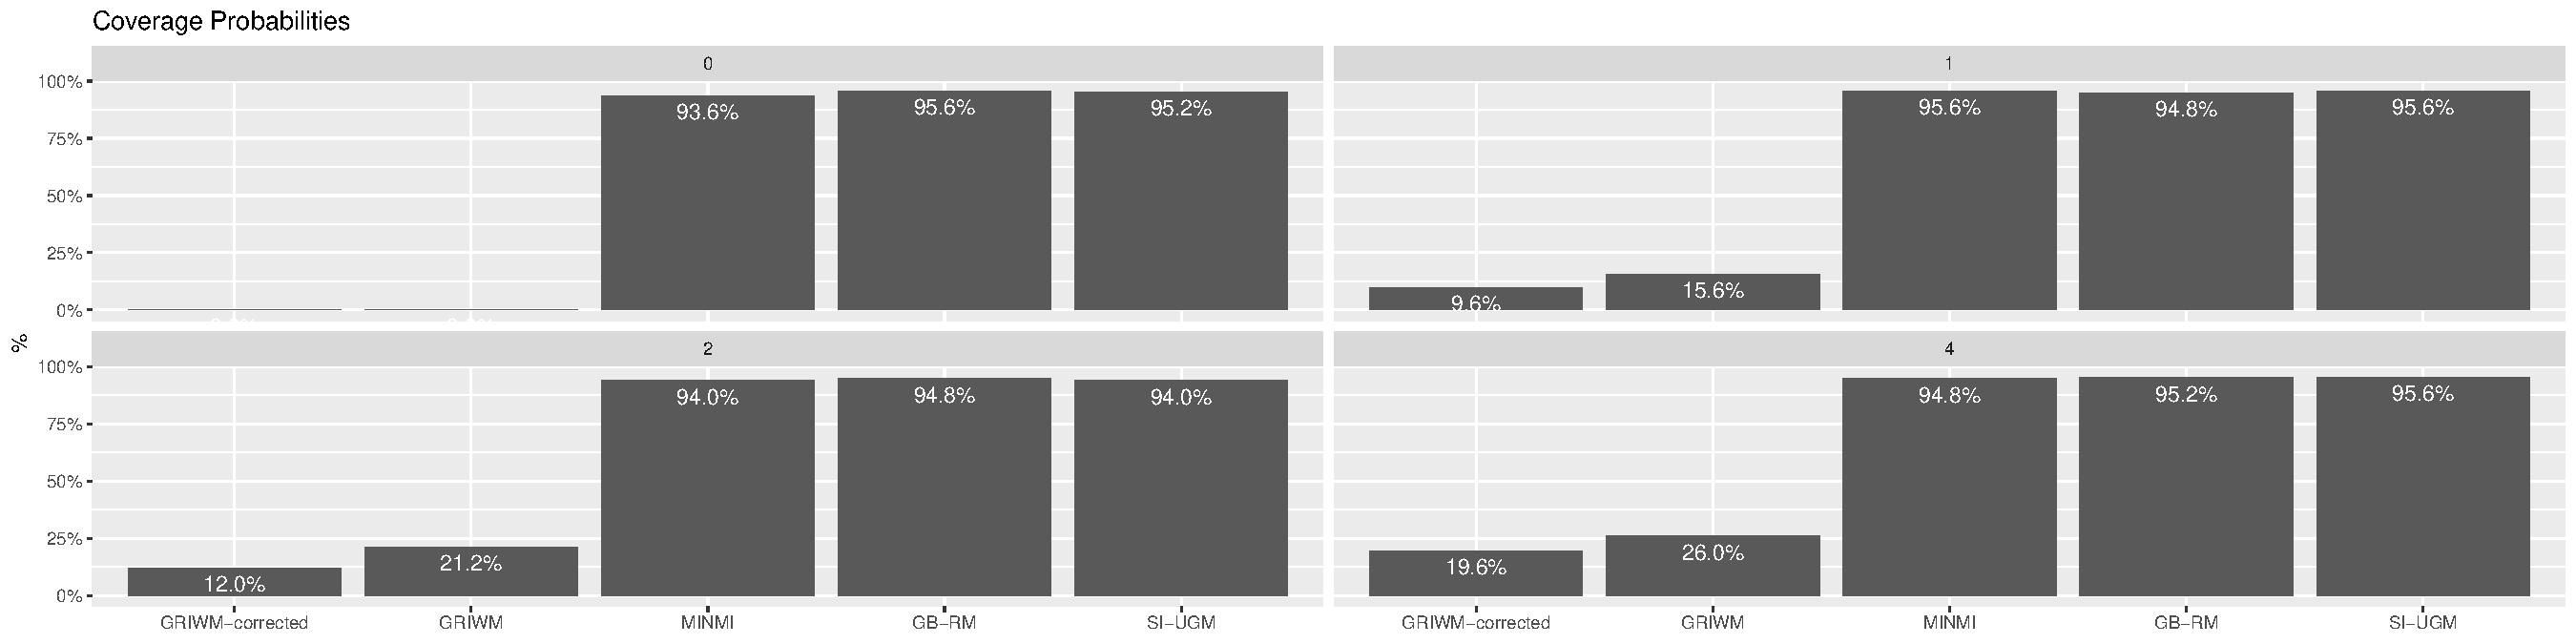
\includegraphics{sim_exp-results_files/figure-latex/unnamed-chunk-7-1.pdf}

\end{document}
